\subsection{$\overline{K_n \cup claw \: m}$}
La familia consiste en un grafo $K_n$ y un grafo claw o estrella formado por un nodo y m nodos adyacentes, 
unidos de forma disjunta, que es luego complementado.
\begin{figure}[H]
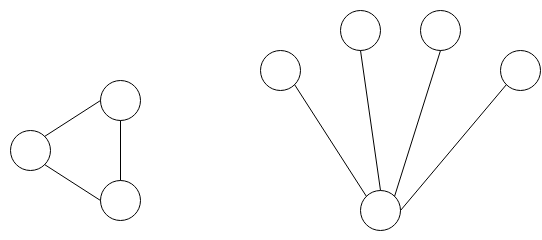
\includegraphics[width=80mm]{K3UC4.png}
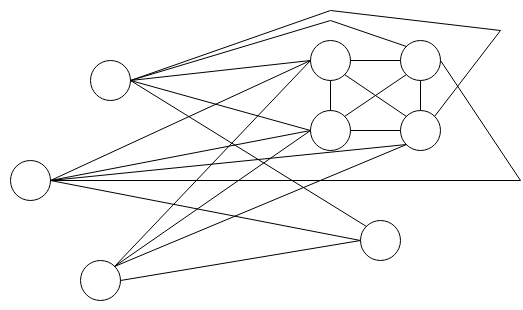
\includegraphics[width=80mm]{K3UC4Complemento.png}
\caption{Ejemplificación: La figura de la izquierda corresponde a $K_3$ $\cup$ $claw$ $4$, 
la figura derecha $\overline{K_3 \cup claw \: 4}$}
\label{overflow}
\end{figure}